{\color{MsBlue} \subsection{\sihao \kaishu \quad \ (一)立项依据与研究内容(建议8000字以下): }}

{\sihao \kaishu \color{MsBlue} 1.{\bfseries 项目的立项依据}(研究意义、国内外研究现状及发展动态分析,需结合科学研究发展趋势来论述科学意义;或结合国民经济和社会发展中迫切需要解决的关键科技问题来论述其应用前景。附主要参考文献目录);}

对于习惯用 \LaTeX 写文档的同学们,一个写基金申请书的模版可能有参考作用。因此我做了这个2021年面上项目申请书正文部分模版。祝大家基金申请顺利!

2023-01-20: 根据2023年面上项目申请书正文的官方MsWord模板,对本模板的字号和少量蓝色文字做了更新。

2023-01-29\&02-01: 根据几位老师的建议,对section的缩进,“参考文献”四个字的大小、字体和居左等做了调整。官方模板中阿拉伯数字不加粗,因此也做了相应的调整。



%\begin{figure}[!th]
%\begin{center}
%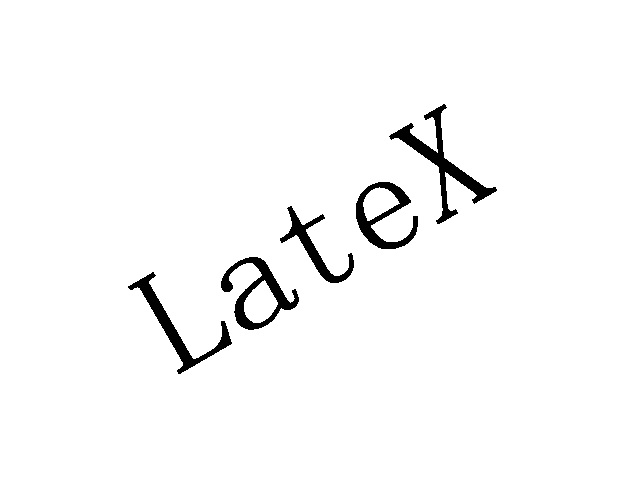
\includegraphics[width=2in]{fig-example.eps}
%\caption{插图可以使用EPS、PNG、JPG等格式。}
%\label{fig:example}
%\end{center}
%\end{figure}

2023-02-06: 根据@Readon的commits,做了如下修改:1. 更正了一处蓝字部分:``(三)其他需要说明的问题'' $\rightarrow$ ``(三)其他需要说明的情况'' 。这个非常重要!2. 设置 AutoFakeBold=3,这样楷体粗体稍微细一点,和官方模板更加接近。3. 调整了页面空白的宽度,大家可以自行微调。作为\LaTeX 菜鸟,非常感谢Readon的专业建议!更多专业的修改请见\url{https://github.com/Readon/NSFC-application-template-latex}



\vskip 2mm
\subsubsection{1.1 声明}
{\bfseries \color{red} 注意!!!非国家自然科学基金委官方模版!!!}由个人根据官方MsWord模版制作。本模版的作者尽力使本模版和官方模版生成的PDF文件视觉效果大致一样,然而,并不保证本模版有用,也不对使用本模版造成的任何直接或间接后果负责。 不得将本模版用于商用或获取经济利益。本模版可以自由修改以满足用户自己的需要。但是如果要传播本模版,则只能传播未经修改的版本。使用本模版意味着同意上述声明。

如有问题,请发送邮件到 \href{mailto:ryanzz@foxmail.com}{ryanzz@foxmail.com}。中了基金的也欢迎反馈。$\smiley$

\subsubsection{1.2 使用说明}\label{sss:instruction}

\begin{enumerate}
\item 编译环境:推荐使用跨平台编译器texlive2017以后的版本,编译顺序为:xelatex+bibtex+xelatex(x2)。windows用户可以用命令行运行批处理文件getpdf.bat,linux用户可以运行runpdf。
\item 本模版力求简单,语句自身说明问题(self explanatory)。几乎只需要修改本tex文件即可满足排版需求,没有sty cls 等文件。用户掌握最基本的\LaTeX 语句即可操作,其余的可以用搜索引擎较容易地获得。
\item 参考文献样式:对作者个数作了限制以适合申请书,当作者个数小于等于5个时,予以全部保留,当作者个数大于5个时,只保留前3个,加et al。参考文献需要放在bib文件中。样式由ieeetrNSFC.bst控制。
\end{enumerate}

\subsubsection{1.3 图、公式和参考文献的引用示例}
尽管不大可能会用到像下面这样简单的公式:
\begin{equation}
\label{eq:ex}
\sqrt[15]{a}=\frac{1}{2},
\end{equation}
我们还是用Eq.(\ref{eq:ex})举个数学公式的例子。同时,我们也不大可能会用到一个长得很像\LaTeX 的图,但是还是引用一下图\ref{fig:example}。图\ref{fig:example}并没有告诉我们关于Jinkela\cite{John1997,Smith1900}的任何信息,也没有透露它的产地\cite{Piter1992}。尽管如此,最近的研究表明,Feizhou非常需要Jinkela\cite{John1997}。
